\chapter{\sffamily Empirical probabilistic reweighting}

{\bfseries\sffamily Concept.} To extend the formalism that we developed in previous chapters to enable the empirical emulation of real-world data via a probabilistic reweighting. This technique should enable a researcher to model complex dynamical trends in the data very well; at the cost of making the abstract interpretation of the model less immediately comprehensible than the statistical inference models in some proceeding chapters. As our generalised framework applies to a wide variety stochastic phenomena, our reweighting algorithm will be applicable to a great breadth of data modeling problems as well. We will also explore some examples which illustrate how the reweighting algorithm should be applied in practice and then follow this up with how the code is designed and implemented as part of a new software package called the `learnadex'. For the mathematically-inclined, this chapter will take a detailed look at how our formalism can be extended to focus on probabilistic reweightings and their optimisation using real-world data. For the programmers, the software described in this chapter lives in the public Git repository: \href{https://github.com/umbralcalc/learnadex}{https://github.com/umbralcalc/learnadex}.

\section{\sffamily Probabilistic formalism}

The key distinction between the methods that we will develop in this chapter and the ones in the proceeding chapters is in their utility when faced with the problem of attempting to model real-world data. In the proceeding chapter, we shall describe some powerful techniques that can be used most effectively when the researcher is aware of the family of models that generated the data. In the present chapter, we will go into the details of how a more `empirical' approach can be derived for dynamical process modeling in a probabilistic framework which locally adapts the model to the data through time. 

While we think that it's worth going into some mathematical detail to give a better sense of where our formalism comes from; we want to emphasise that the framework we discuss here is not new to the technical literature at all. Our overall framework draws on influences from Empirical Dynamical Modeling (EDM)~\cite{sugihara1990nonlinear}, some classic nonparametric local regression techniques --- such as LOWESS/Savitzky-Golay filtering~\cite{savitzky1964smoothing} --- and also Gaussian processes~\cite{murphy2012machine} as well. The novelties here, instead, lie more in the specifics of how we combine some of these ideas together when referencing the stochadex formalism, and how this manifests in designing more generally-applicable software for the user.

Before we are able to develop this empirical reweighting algorithm, we need to return to the stochadex formalism that we introduced in the first chapter of this book. As we discussed at that point; this formalism is appropriate for sampling from nearly every stochastic phenomenon that one can think of. However, when trying robustly assess how far a model is from accurately describing a set of real-world data, trying to use only generated samples of the model process can be diffcult. Instead, in this section, we are going to extend this formalism to look at how probability theory can help with this data comparison problem in a systematic way.

\begin{figure}[h]
\centering
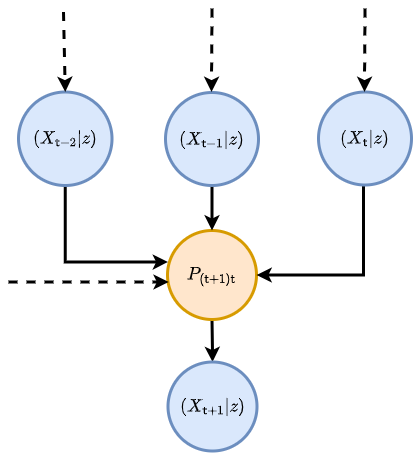
\includegraphics[width=8cm]{images/chapter-4-master-eq-graph.drawio.png}
\caption{Graph representation of Eq.~(\ref{eq:master-x-cont}).}
\label{fig:master-eqn}
\end{figure} 

So, how do we begin? In the first chapter, we defined the general stochastic process with the formula $X^{i}_{{\sf t}+1} = F^{i}_{{\sf t}+1}(X',z,{\sf t})$. This equation also has an implicit \emph{master equation} associated to it that fully describes the time evolution of the \emph{probability density function} $P_{{\sf t}+1}(x\vert z)$ of the next matrix row being $x=X_{{\sf t}+1}$ given that the parameters of the process are $z$. This can be written as
%%
\begin{align}
P_{{\sf t}+1}(x\vert z) &= \frac{1}{{\sf t}}\sum_{{\sf t}'=0}^{{\sf t}}\int_{\omega_{{\sf t}'}}{\rm d}x' P_{{\sf t}'}(x'\vert z) P_{({\sf t}+1){\sf t}'}(x\vert x',z) \label{eq:master-x-cont} \,,
\end{align}
%%
where at the moment we are assuming the state space is continuous in each dimension and $P_{({\sf t}+1){\sf t}'}(x\vert x',z)$ is the conditional probability that the matrix row at time $({\sf t}+1)$ will be $x=X_{{\sf t}+1}$ given that the row at time ${\sf t}'$ was $x'=X_{{\sf t}'}$ and the parameters of the process were $z$. This is a very general equation which should almost always apply to any continuous stochastic phenomenon we want to study in due course. To try and understand what this equation is saying we find it's helpful to think of an iterative relationship between probabilities; each of which is connected by their relative conditional probabilities. This kind of thinking is also illustrated in Fig.~\ref{fig:master-eqn}.

The factor of $1/{\sf t}$ in Eq.~(\ref{eq:master-x-cont}) is a normalisation factor --- this just normalises the sum of all probabilities to 1 given that there is a sum over ${\sf t}'$. Note that, if the process is defined over continuous time, we would need to replace 
%%
\begin{align}
\frac{1}{{\sf t}}\sum_{{\sf t}'=0}^{{\sf t}} \rightarrow \frac{1}{t({\sf t})}\sum_{{\sf t}'=0}^{{\sf t}}\delta t({\sf t}') \,.
\end{align}
%% 
But what is $\omega_{\sf t}$? You can think of this as just the domain of possible $x'$ inputs into the integral which will depend on the specific stochastic process we are looking at.

If we wanted to compute the mean of the distribution $M_{{\sf t}+1}(z)$ in Eq.~(\ref{eq:master-x-cont}), it would be straightforward to just multiply both sides of the expression by $x$ and integrate over ${\rm d}x$ in the $\omega_{{\sf t}+1}$ domain. However, there is another similar expression for the mean that we can derive under certain conditions which will be valuable to us when developing the empirical reweighting. If the probability distribution is \emph{stationary} --- meaning that $P_{{\sf t}'}(x\vert z)=P_{{\sf t}''}(x\vert z)$ for all ${\sf t}'$ and ${\sf t}''$ --- it's possible to derive\footnote{To see that this is true, first note that the joint distribution $P_{({\sf t}+1){\sf t}'}(x,x'\vert z)=P_{({\sf t}+1){\sf t}'}(x\vert x',z)P_{{\sf t}'}(x'\vert z)$. Secondly, note that joint distributions always allow variable swaps trivially like this $P_{({\sf t}+1){\sf t}'}(x,x'\vert z)=P_{{\sf t}'({\sf t}+1)}(x',x\vert z)$. Then, lastly, note that stationarity of $P_{{\sf t}+1}(x\vert z)=P_{{\sf t}'}(x\vert z)$ means 
$$\int {\rm d}x\int {\rm d}x' \, x\,P_{({\sf t}+1){\sf t}'}(x,x'\vert z)=\int {\rm d}x\int {\rm d}x'  \, x\, P_{{\sf t}'({\sf t}+1)}(x,x'\vert z)=\int {\rm d}x\int {\rm d}x'  \, x\, P_{({\sf t}+1){\sf t}'}(x',x\vert z)\,,$$
where we've used the trivial variable swap to get to the last equality, and the domain references $\omega$ in the integrals are implicitly defined.} 
%%
\begin{align}
M_{{\sf t}+1}(z) = \int_{\omega_{{\sf t}+1}}{\rm d}x \,x\,P_{{\sf t}+1}(x\vert z) &= \frac{1}{{\sf t}}\sum_{{\sf t}'=0}^{{\sf t}}\int_{\omega_{{\sf t}'}}{\rm d}x'\int_{\omega_{{\sf t}+1}}{\rm d}x \, x' \, P_{{\sf t}'}(x'\vert z) P_{({\sf t}+1){\sf t}'}(x\vert x',z) \label{eq:stationary-mean-estimator}\,.
\end{align}
%%
The standard covariance matrix elements can also be computed in a similar fashion
%%
\begin{align}
C^{ij}_{{\sf t}+1}(z) &= \int_{\omega_{{\sf t}+1}}{\rm d}x \,[x-M_{{\sf t}+1}(z)
]^i[x-M_{{\sf t}+1}(z)]^jP_{{\sf t}+1}(x\vert z) \nonumber \\
&= \frac{1}{{\sf t}}\sum_{{\sf t}'=0}^{{\sf t}}\int_{\omega_{{\sf t}'}}{\rm d}x'\int_{\omega_{{\sf t}+1}}{\rm d}x \, [x'-M_{{\sf t}+1}(z)]^i[x'-M_{{\sf t}+1}(z)]^j P_{{\sf t}'}(x'\vert z) P_{({\sf t}+1){\sf t}'}(x\vert x',z) \label{eq:stationary-covariance-estimator}\,.
\end{align}
%%

While they look quite abstract, Eqs.~(\ref{eq:stationary-mean-estimator}) and~(\ref{eq:stationary-covariance-estimator}) express the core idea behind how our probabilistic reweighting will function. By assuming a stationary distribution, we gain the ability to directly estimate the statistics of the probability distribution $P_{{\sf t}+1}(x\vert z)$ from past samples it may have in empirical data; which are represented here by $P_{{\sf t}'}(x'\vert z)$.

In order to study higher-order out-of-time-order correlations, we can also consider using the statistical moments computed from joint distributions like these
%%
\begin{align}
P_{({\sf t}+1){\sf t}'}(x, x'\vert z) &= P_{({\sf t}+1){\sf t}'}(x\vert x',z)P_{{\sf t}'}(x'\vert z) \label{eq:2nd-joint-dist}\\
P_{({\sf t}+1){\sf t}'{\sf t}''}(x, x', x''\vert z) &= P_{({\sf t}+1){\sf t}'{\sf t}''}(x\vert x', x'', z)P_{{\sf t}'{\sf t}''}(x'\vert x'', z)P_{{\sf t}''}(x''\vert z) \label{eq:3rd-joint-dist}\,.
\end{align}
%%
For example, Eq.~(\ref{eq:2nd-joint-dist}) would apply if we wanted to retrieve the out-of-time-order pairwise correlations between $x$ at timestep ${\sf t}+1$ and $x'$ at timestep ${\sf t}'$. Using this pairwise relationship we can also derive an equation for the out-of-time-order covariance matrix elements
%%
\begin{align}
C_{({\sf t}+1){\sf t}'}^{ij}(z) &= \frac{1}{{\sf t}}\sum_{{\sf t}'=0}^{{\sf t}}\int_{\omega_{{\sf t}'}}{\rm d}x'\int_{\omega_{{\sf t}+1}}{\rm d}x \,[x-M_{{\sf t}+1}(z)]^i[x'-M_{{\sf t}'}(z)]^j P_{({\sf t}+1){\sf t}'}(x, x'\vert z) \label{eq:out-of-time-order-covariance-estimator} \,.
\end{align}
%%

What other processes can be described by Eq.~(\ref{eq:master-x-cont})? For Markovian phenomena, the equation no longer depends on timesteps older than the immediately previous one, hence the expression reduces to just
%%
\begin{align}
P_{{\sf t}+1}(x\vert z) &= \int_{\omega_{\sf t}}{\rm d}x' P_{\sf t}(x'\vert z) P_{({\sf t}+1){\sf t}}(x\vert x',z) \label{eq:master-x-cont-markov} \,.
\end{align}
%%
An analog of Eq.~(\ref{eq:master-x-cont}) exists for discrete state spaces as well. We just need to replace the integral with a sum and the schematic would look something like this
%%
\begin{align}
P_{{\sf t}+1}(x\vert z) &= \frac{1}{{\sf t}}\sum_{{\sf t}'=0}^{\sf t}\sum_{\omega_{{\sf t}'}} P_{{\sf t}'}(x'\vert z) P_{({\sf t}+1){\sf t}'}(x \vert x', z) \label{eq:master-x-disc} \,,
\end{align}
%%
where we note that the $P$'s in the expression above all now refer to \emph{probability mass functions}. In the even-simpler case where $x$ is just a vector of binary `on' or `off' states, Eq.~(\ref{eq:master-x-disc}) reduces to
%%
\begin{align}
P^i_{{\sf t}+1}(z) &= \frac{1}{{\sf t}}\sum_{{\sf t}'=0}^{\sf t} \sum_{j=1}^d P^j_{{\sf t}'}(z) P^{ij}_{({\sf t}+1){\sf t}'}(z) \nonumber \\
&= \frac{1}{{\sf t}}\sum_{{\sf t}'=0}^{\sf t} \sum_{j=1}^d \big\{ P^j_{{\sf t}'}(z) A^{ij}_{({\sf t}+1){\sf t}'}(z) + [1-P^j_{{\sf t}'}(z)] B^{ij}_{({\sf t}+1){\sf t}'}(z) \big\} \label{eq:master-x-disc-binary}\,,
\end{align}
%% 
where $P^i_{{\sf t}'}(z)$ now represents the probability that element $x^i=1$ (is `on') at time ${\sf t}'$ given $z$. We've also implicitly defined the matrices $A$ and $B$ as the conditional probabilities where the previous state in time $P^j_{{\sf t}'}(z)$ was either `on' or `off', respectively.

In this section, we looked into how the mathematical formalism used in the stochadex could be extended with probability theory. Now that we have more of a sense of how this formalism works, we are ready to move on to designing the algorithm for our reweighting. So let's go!

\section{\sffamily Generalised reweighting algorithm}

The empirical probabilistic reweighting algorithm that we're going to describe in this section will depend on the stationarity of $P_{{\sf t}+1}(x\vert z)=P_{{\sf t}'}(x\vert z)$ such that, e.g., Eq.~(\ref{eq:stationary-mean-estimator}) is applicable. But before we think about the various kinds of conditional probability we could use in the reweighting, we need to connect values of $x$ in our reweighting to the data from which it will be learning. 

If the mean is a sufficient statistic for the distribution which describes the data, a choice of, e.g., Exponential, Poisson or Binomial distribution could be used where the mean is estimated directly from the time series using Eq.~(\ref{eq:stationary-mean-estimator}), given a conditional probability $P_{({\sf t}+1){\sf t}'}(x\vert x',z)$. Extending this idea further to include distributions which also require a variance to be known, e.g., the Normal, Gamma or Negative Binomial distributions could be used where the variance (and/or covariance) could be estimated using Eq.~(\ref{eq:stationary-covariance-estimator}). These are just a few simple examples of distributions that can link the estimated statistics from Eqs.~(\ref{eq:stationary-mean-estimator}) and~(\ref{eq:stationary-covariance-estimator}) to a time series dataset. However, the algorithmic framework is very general to whatever choice of `data linking' distribution that a researcher might need.

We should probably make what we've just said a little more mathematically concrete. Let's define a data vector $y=Y_{{\sf t}+1}$ at time ${\sf t}+1$, which shares the same length as $x$, and represents a specific observation of $x$ at this point in a real dataset. At this point in time, we can define $P_{{\sf t}+1}[y{=}Y_{{\sf t}+1};M_{{\sf t}+1}(z),C_{{\sf t}+1}(z),\dots ]$ as representing the likelihood of $y=Y_{{\sf t}+1}$ given the estimated statistics from Eqs.~(\ref{eq:stationary-mean-estimator}) and~(\ref{eq:stationary-covariance-estimator}) (and maybe higher-orders). Note that in order to do this, we need to identify the $x'$ and ${\sf t}'$ values that are used to estimate, e.g., $M_{{\sf t}+1}(z)$ with the past data values which are observed in the dataset time series itself. Now that we have this likelihood, we can immediately evaluate an objective function (a cumulative log-likelihood) that we might seek to optimise over for a given dataset 
%%
\begin{align}
\ln {\cal L}_{{\sf t}+1}(Y\vert z) = &\ln P_{{\sf t}+1}[y{=}Y_{{\sf t}+1};M_{{\sf t}+1}(z),C_{{\sf t}+1}(z),\dots ] + \ln P_{{\sf t}}[y{=}Y_{{\sf t}};M_{{\sf t}}(z),C_{{\sf t}}(z),\dots ] + ... \,, \label{eq:log-likelihood-reweighting}
\end{align}
%%
where the summation continues until all of the past measurements $Y_{{\sf t}+1}, Y_{{\sf t}}, \dots$ which exist as rows in the data matrix $Y$ have been taken into account.

\begin{figure}[h]
\centering
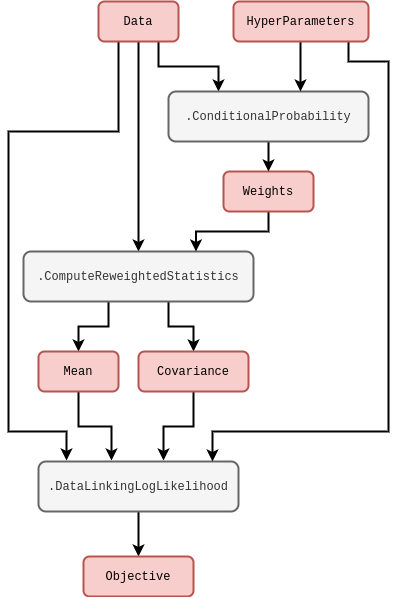
\includegraphics[width=8cm]{images/chapter-4-prob-reweighting-code.drawio.png}
\caption{Code schematic of the probability reweighting optimisation.}
\label{fig:prob-reweighting-code}
\end{figure} 

By optimising Eq.~(\ref{eq:log-likelihood-reweighting}) with respect to all of the hyperparameters $z$, we are effectively adopting what is known as an `empirical Bayes' approach~\cite{murphy2012machine, mackay2003information}. We might think of the overall generalised reweighting algorithm as the code schematic in Fig.~\ref{fig:prob-reweighting-code}.

In order to specify what $P_{({\sf t}+1){\sf t}'}(x\vert x',z)$ is, it's quite natural to define a set of hyperparameters for the elements of $z$. To get a sense of how the data-linking function relates to these hyperparameters, it's instructive to consider an example. One generally applicable option for the conditional probability could be a purely time-dependent covariance kernel matrix
%%
\begin{align}
P_{({\sf t}+1){\sf t}'}(x\vert x',z)\,{\rm d}x\, {\rm d}x' &\propto K^{-1}(z, {\sf t}+1,{\sf t}')  \label{eq:time-dependent-kernel} \,, 
\end{align}
%%
and the data-linking distribution, e.g., could be a Gaussian
%%
\begin{align}
P_{{\sf t}+1}[y{=}Y_{{\sf t}+1};M_{{\sf t}+1}(z),C_{{\sf t}+1}(z),\dots ] = {\sf MultivariateNormalPDF}[y{=}Y_{{\sf t}+1};M_{{\sf t}+1}(z),C_{{\sf t}+1}(z)] \label{eq:gaussian-data-prob}\,.
\end{align}
%%

In the case of Eqs.~(\ref{eq:time-dependent-kernel}) and~(\ref{eq:gaussian-data-prob}) above, the hyperparameters that would be optimised could relate to the kernel in a wide variety of ways. Optimising them would make our optimised reweighting very similar to (but not quite the same as) evaluating maximum a posteriori (MAP) of a Gaussian process regression. The main differences here are that the mean of a Gaussian process as a function of time is typically included within $z$, and hence must be obtained through optimisation. In contrast, our methodology relies on the fact that the mean estimator can be computed directly by weighted sample estimation and can then be fed to some data-linking distribution. By doing it this way, we enable many different kinds of data to be described by the same underlying conditional probability-based reweighting and also make incorporating future data into the current model much easier then is the case for a standard Gaussian process (which would require re-optimising with respect to the next data point every time). The time-dependent kernel we have chosen in Eq.~(\ref{eq:time-dependent-kernel}) also only represents one particular choice, but we could consider a wide range of state-dependent conditional probability weightings for the algorithm as well. 

As another form of flexibility; we could also try adapting the data-linking distributions to include an intercept term and linear coefficients for the statistics which are passed to it. These could then be treated as additional hyperparameters and optimised jointly with the others if there is sufficient constraining power in the data.

The optimisation approach that we choose to use for obtaining the best hyperparameters in the conditional probability of Eq.~(\ref{eq:log-likelihood-reweighting}) will depend on a few factors. For example, if the number of hyperparameters is relatively low, but their gradients are difficult to calculate exactly; then a gradient-free optimiser (such as the Nelder-Mead~\cite{nelder1965simplex} method or something like a particle swarm~\cite{kennedy1995particle, shi1998modified}) would likely be the most effective choice. On the other hand, when the number of hyperparameters ends up being relatively large, it's usually quite desriable to utilise the gradients in algorithms like vanilla Stochastic Gradient Descent~\cite{robbins1951stochastic} (SGD) or Adam~\cite{kingma2014adam}.

If the gradients of Eq.~(\ref{eq:log-likelihood-reweighting}) are needed, we can always factorise each derivative with respect to hyperparameter $z^i$ in the following way through the chain rule
%%
\begin{align}
\frac{\partial}{\partial z^i}\ln {\cal L}_{{\sf t}+1}(Y \vert z) &= \frac{\partial M_{{\sf t}+1}}{\partial z^i}\frac{\partial}{\partial M_{{\sf t}+1}}\ln P_{{\sf t}+1}[y{=}Y_{{\sf t}+1};M_{{\sf t}+1}(z),C_{{\sf t}+1}(z),\dots ] \nonumber \\ 
&\qquad + \frac{\partial C_{{\sf t}+1}}{\partial z^i}\frac{\partial }{\partial C_{{\sf t}+1}}\ln P_{{\sf t}+1}[y{=}Y_{{\sf t}+1};M_{{\sf t}+1}(z),C_{{\sf t}+1}(z),\dots ] + \dots  \,. \label{eq:log-likelihood-reweighting-grad}
\end{align}
%%
By factoring derivatives in this manner, the computation can be separated into two parts: the derivatives with respect to $M_{{\sf t}+1}$ and $C_{{\sf t}+1}$, which are typically quite straightforward; and the derivatives with respect to $z$ elements, which typically need a more involved calculation depending on the model. Incidentally, this separation also neatly lends itself to abstracting gradient calculations as having a simpler, general purpose component that can be built directly into a library of data models and a more complex, model-specific component that the user must specify.

\section{\sffamily Software design}

Let's now take a step back from the specifics of the probabilistic reweighting algorithm to introduce our new sofware package for this part of the book: the `learnadex'. At its core, the learnadex algorithm adapts the stochadex iteration engine to iterate through streams of data in order to accumulate a global objective function value with respect to that data. The user may then choose which optimisation algorithm (or write their own) to use in order to leverage this objective for learning a better representation of the data. Readers with some familiarity of machine learning concepts will note that this design should enable either `offline' or `online' learning algorithms to work.

Using the iteration engine of the stochadex makes neat use of software which has already been designed and tested in earlier chapters of this book. However, in order to fully achieve this, a few minor extensions to the typing structures and code abstractions are necessary; as we show in Fig.~\ref{fig:learnadex-data-types-design}. To start with, we separate out `learning' from the kind of optimiser in the overall config so as to enable multiple optimisation algorithms to be used for the same learning problem. The hyperparameters that define that optimisation problem domain can be determined by the user with an extension to the \texttt{OtherParams} object so that it includes some optional Boolean masks over the parameters, i.e., \texttt{OtherParams.FloatParamMask} and \texttt{OtherParams.IntParamMask}. These masks are used to extract the parameters of interest, which can then be flattened and formatted to fit into any generic optimisation algorithm.

\begin{figure}[h]
\centering
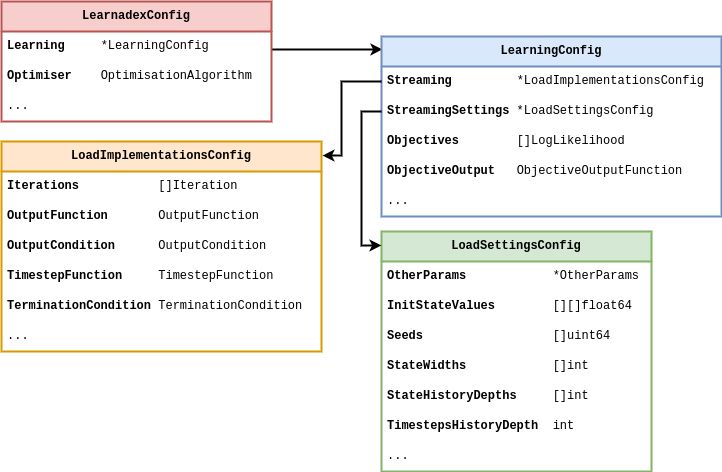
\includegraphics[width=12cm]{images/chapter-4-learnadex-data-types.drawio.png}
\caption{A relational summary of the core data types in the learnadex.}
\label{fig:learnadex-data-types-design}
\end{figure}

On the learning side; in order to define a specific objective for each data iterator to compute while the data streams through it, we have abstracted a `log-likelihood' type. Similarly, each iterator also gets a data streamer configuration which defines where the data is streaming from --- e.g., from a file on disk, from a local database instance or maybe via a network socket --- and also some inherited abstractions from the stochadex which define the time stepping function and when the data stream ends. In Fig.~\ref{fig:learnadex-data-iterator} below, we provide a schematic of the method calls of (and within) each data iterator.

\textcolor{red}{\begin{itemize}
\item{describe the method calls diagram in more detail --- in particular, point out how it can replace the \texttt{Iteration.Iterate} method which is called when the \texttt{StateIterator} is asked for another iteration from the \texttt{PartitionCoordinator} of the stochadex}
\item{then talk about the optimiser! starting with non-gradient-based: the two packages that are supported out of the box are gonum and eaopt (still need to do gago --- see here: github.com/maxhalford/eaopt) }
\item{then talk about the output - talk about the possibilities for output and what the default setting to json logs is for}
\item{could also be written to, e.g., a locally-hosted database server and the best-suited would be a NoSQL document database, e.g., MongoDB~\cite{mongodb}, but building something bespoke and simpler is more aligned with the use-case here and with the principles of this book}
\item{describe the need for log exploration and visualisation and then introduce logsplorer - a REST API for querying the json logs (with basic filtering and selection capabilities but could be extended to more advanced options) and optionally also launches a visualisation React app written in Typescript}
\item{note how this could be scaled to cloud services easily and remotely queried through the logsplorer API and visualised} 
\end{itemize}}

\begin{figure}[h]
\centering
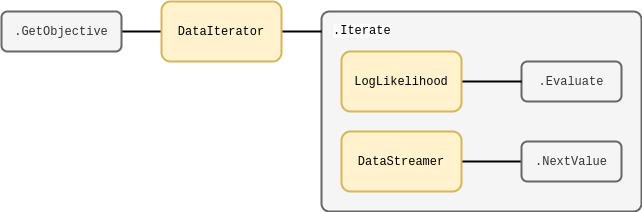
\includegraphics[width=14cm]{images/chapter-4-learnadex-data-iterator.drawio.png}
\caption{A schematic of an iteration with an objective function evaluation.}
\label{fig:learnadex-data-iterator}
\end{figure}

As with the software we wrote for the stochadex, the learnadex main binary executable leverages templating to enable full configurability of all the implementations and settings of Fig.~\ref{fig:learnadex-data-types-design} through passing configs at runtime. Users can alternatively use the learnadex as a library for import, if they desire more control over the code execution. 

\begin{figure}[h]
\centering
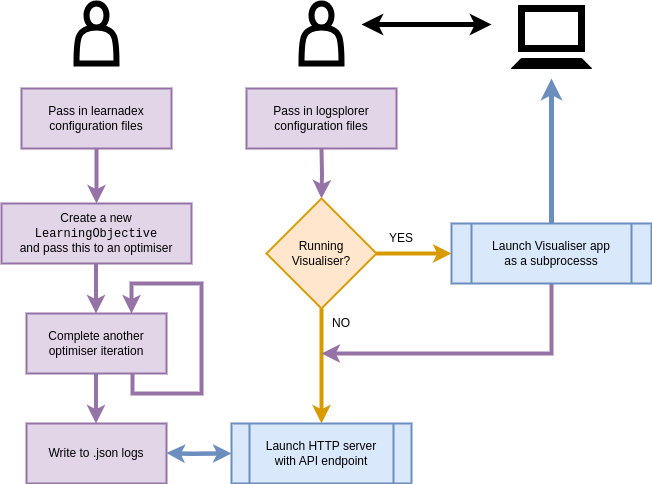
\includegraphics[width=13cm]{images/chapter-4-learnadex-main.drawio.png}
\caption{A diagram of the main learnadex and logsplorer executables.}
\label{fig:learnadex-main}
\end{figure}
    